%!TEX root = ../main.tex
%%=====================================================================
%%  §4  WHAT GROUPING BUYS: THE HEDGE AND THE SIGNAL         target 4-5 pp.
%%      THE PAPER'S MAIN RESULT SECTION.
%%
%%  Three movements, in this order:
%%
%%  5.1  THE DISPERSION CONTRAST. Across the field the alpha against
%%       FF5+MOM is narrow and the volatility is not.
%%         alpha  6.085 - 7.689 %/yr   (cv 5.5%)
%%         vol    2.434 - 4.584 %/yr   (cv 18.8%)
%%       Report the one-way ANOVA using the seed replicates as the
%%       within-group variation, and make the point as a MAGNITUDE
%%       CONTRAST (between/within sd ratio ~3.03 for volatility against
%%       ~1.12 for alpha).
%%       ⛔ Do NOT claim the alphas are equal. That null is REJECTED:
%%          F = 3.775, p = 2.546e-4.
%%
%%  5.2  THE SAME CONTRAST ONE LAYER DOWN -- this is what settles whether
%%       the asymmetry belongs to the clustering or to the trained model.
%%         rule-based layer   alpha cv 7.9%   vol cv 18.2%   ratio 2.30x
%%         trained layer      alpha cv 5.5%   vol cv 18.8%   ratio 3.42x
%%       The asymmetry survives the change of layer, so it is not an
%%       artefact of the head.
%%       ⚠ BUT THE SECOND READING MUST BE IN THE SAME PARAGRAPH: at the
%%       rule-based layer the two controls hold the two LOWEST alphas of
%%       the twenty-one (6.066 and 6.314 against 8.729 for the best), so
%%       clustering there improves BOTH moments, unequally. Flatness of
%%       alpha is a TRAINED-LAYER statement. Scope it every time.
%%       ⛔ Print no cross-layer alpha LEVEL difference: the two books
%%          run 5-day and 30-day signal windows at different gross
%%          conventions. Only WITHIN-layer dispersion is clean.
%%       Source: scripts/naive_spanning.csv, NUMBERS.md N12.5.
%%
%%  5.3  THE EXACT DECOMPOSITION. Since log SR = log mean - log vol,
%%       var(log SR) splits additively with no residual:
%%         return 18.1%,  volatility 81.9%   (SET19, realized pairing)
%%         return 13.5%,  volatility 86.5%   (alpha pairing)
%%       The volatility share is robust across arm sets (72-86%).
%%       ⚠ corr(log mean, log vol) is -0.3228 on the nineteen and
%%         +0.3781 on the twelve methods alone. THE SIGN FLIPS WITH THE
%%         ARM SET. Every sentence using it names its set, and
%%         "the variance reduction is not paid for in return" may NOT be
%%         stated unconditionally.
%%
%%  Point forward to §4 for why the dispersion comparison is meaningful:
%%  the precision argument licenses reading these spreads at all.
%%
%%  FIGURES: fig_alpha_vol, fig_variance_share.
%%
%%  RETIRED AND REMOVED -- do not reinstate: the era rank-stability
%%  asymmetry (vol Spearman +0.86 vs alpha +0.02). Both halves fail.
%%  See §4.4 and NUMBERS.md N5, N5.1, N5.2.
%%=====================================================================
\section{Decomposing Portfolio Performance}
\label{sec:riskreturn}
%%  TITLE SETTLED 2026-08-23. §6 (the trading head) was folded in as
%%  §4.4, so the heading names the object measured rather than the
%%  clustering alone.

In this section, we show that a real partition lowers the volatility of the payoff and raises its alpha. We measure both effects within each trading component. We then measure the variance share of each partition, the share of the cross-sectional variance of the day's market residuals that demeaning within its groups removes. For a random partition, we show that this variance share equals the degrees-of-freedom floor, the variance share that $\K$ random groups remove in expectation (\secref{sec:mechanism}). Next, we decompose the Sharpe gap between the clusterizers' portfolios and the control portfolios into a mean part and a volatility part (\secref{sec:split}). Finally, we hold the partition fixed and measure what the neural trading head adds to the performance (\secref{sec:head}).

%%  ── 4.0  OPENING ────────────────────────────────────────────────────
%%  Two goods, priced separately. Then the licence, pointing at §3.6.
%%  DRAFTED WORDING (already in the abstract and §1, keep consistent):
%%    hedge  = book runs ~two fifths less volatile than either control
%%             under the fixed rule (42/39%) and ~a third under the head
%%             (31/33%). CORRECTED 2026-08-23: the earlier note said "a
%%             third at BOTH components, training barely narrows it".
%%             Both halves were wrong; tab:hedge's own cells give the
%%             split, and 04:89 already prints the honest 28-42% band.
%%    signal = controls hold the lowest alphas at the rule-based layer;
%%             training halves the advantage over K=1 (pre-2009) and
%%             leaves the advantage over random untouched
%%    -> the model substitutes for a MISSING clustering, not a WRONG one


\subsection{The Alpha and Volatility}
\label{sec:hedge}

We find that clustering lowers portfolio volatility by $28\%$ to $42\%$ in every combination of trading component, control, and averaging convention across head seeds (\tabref{tab:moments} and its notes). In both trading components, each control portfolio is much more volatile than any of the 12 clusterizers' portfolios. Although the volatility reduction is smaller in the trained trading component than in the rule-based trading component, it persists against both controls. Against the $\K=1$ control, the reduction is $41.9\%$ in the rule-based component and $35.4\%$ in the trained component. Against the random control, it is $38.7\%$ in the rule-based component and $33.0\%$ in the trained component. The lower end of the range, $28\%$, comes from averaging the trained payoffs over head seeds before measuring their volatility (notes to \tabref{tab:moments}).

%%=====================================================================
%%  v3 UPDATE, 2026-08-20 -- PARTIAL, BY DESIGN.
%%  APPLIED (each recomputed from source in this session, not relayed):
%%    tab:hedge trained row, tab:signal trained row, the forty-two-run
%%    no-overlap sentence, the band-gap sentence, the day counts.
%%  ⛔ NOT APPLIED, and every one of these is still an OLD-PANEL number:
%%    - every RULE-BASED cell in both tables, and the "31 to 40%" band at
%%      :89, the "training narrows" sentence at :91, and the rules'-mean
%%      parenthetical at :213. All need the v3 naive per-day books, which
%%      did not exist until today (run_naive_routeA.py wrote only a
%%      summary CSV); they are landing in naive_routeA/daily_v3/.
%%    - the comovement-removed band at :245/:247/:255. The ledger's v3
%%      values are SINGLE-SOURCE and live only in scratch; :245's printed
%%      "17.5-20.2%" survives only under two undisclosed choices (drop
%%      GICS, and leave singletons untouched). Do not print until the
%%      measurement is persisted and reproduced.
%%    - the variance-share figures at :306/:309. The "no cell below 62%"
%%      floor is reported BROKEN on v3 (four GICS cells, min 51%), but
%%      that is not yet independently reproduced here.
%%  ⚠ :258 "its book is the most volatile in the field" is a
%%    PRE-EXISTING internal contradiction, not a v3 change: true at the
%%    trained component, false at the rule-based one, where tab:hedge
%%    says so 150 lines earlier.
%%=====================================================================
\begin{table}[tb]
\centering
\caption{Portfolio volatility and factor alpha: 12 clusterizers against the two
controls, within each trading component}
\label{tab:moments}
\begin{threeparttable}
\small
\setlength{\tabcolsep}{4pt}
\begin{tabular}{@{}llccccc@{}}
\toprule
& & \multicolumn{3}{c}{Level (\%/yr)} &
  \multicolumn{2}{c}{Change from clustering} \\
\cmidrule(lr){3-5}\cmidrule(lr){6-7}
& Trading component & 12 clusterizers & $\K=1$ & Random & against $\K=1$ & against Random \\
\midrule
Volatility & Rule-based & $2.38$--$3.09$ & $4.65$ & $4.41$ & $-41.9\%$ & $-38.7\%$ \\
           & Trained & $2.88$--$3.80$ & $5.07$ & $4.89$ & $-35.4\%$ & $-33.0\%$ \\
\addlinespace
Alpha      & Rule-based & $4.03$--$4.40$ & $3.63$ & $3.72$ & $+15.6\%$ & $+13.1\%$ \\
           & Trained & $5.89$--$7.02$ & $5.44$ & $5.33$ & $+20.0\%$ & $+22.5\%$ \\
\bottomrule
\end{tabular}
\begin{tablenotes}[flushleft]\small
\item \emph{Notes.} This table reports the annualized volatility and the annualized alpha of the rule-based and trained portfolios of the 12 clusterizers and the two controls, and the change from each control's level to the clusterizers'. All 14 configurations of each trading component are measured on the $6{,}913$-day sample of \secref{sec:panel} (July 1997 to December 2024), with the common 60-day estimation window wherever the partition is estimated from returns or correlations. Both trading components have gross exposure one (\secref{sec:components}). Alphas are against the Fama--French five factors \citep{fama2015five} plus momentum \citep{carhart1997persistence} (FF5+MOM below), with Newey--West(21) standard errors. Each payoff is paired with the factor return of the calendar day on which it was realized. Each trading component is joined to the factor file on its own realization calendar (\appref{app:calendar}). Trained volatilities are computed per head seed and averaged over the five head seeds. Trained alphas are estimated on the payoff averaged over the five head seeds. For alpha, the two conventions give the same point estimate, because an OLS intercept is linear in the dependent variable. Change is the ratio of the 12 clusterizers' mean level to the level of the control, minus one, computed on unrounded values. For volatility, those means are $2.70$ in the rule-based component and $3.27$ in the trained component. For alpha, they are $4.20$ in the rule-based component and $6.52$ in the trained component. Averaging the trained payoff series over head seeds before measuring volatility gives $2.66$--$3.48$ for the clusterizers. On this convention, the volatility is $4.44$ for the $\K=1$ control and $4.18$ for the random control. The changes are then $-32.3\%$ against the $\K=1$ control and $-28.1\%$ against the random control.
\end{tablenotes}
\end{threeparttable}
\end{table}

For the neural trading head, the volatility of the 12 clusterizers' portfolios ranges from $2.88\%$ for $k$-means on returns to $3.80\%$ for unsigned spectral clustering. This band is $0.9$ percentage points wide. Each control's volatility is about a percentage point above the top of this band. Across the 12 trained portfolios, the highest volatility is $32\%$ above the lowest, whereas the highest alpha is $19\%$ above the lowest (\tabref{tab:moments}). The Sharpe ratios of these portfolios therefore differ mainly through volatility. \figref{fig:alpha_vol} plots alpha against volatility for the trained portfolios. Both control portfolios lie outside the ranges of the 12 clusterizers' portfolios, with lower alpha and higher volatility. The rule-based portfolios show the same pattern. In \secref{sec:invariance}, we return to how little the choice of clusterizer affects the results downstream.

\begin{figure}[tb]
\centering
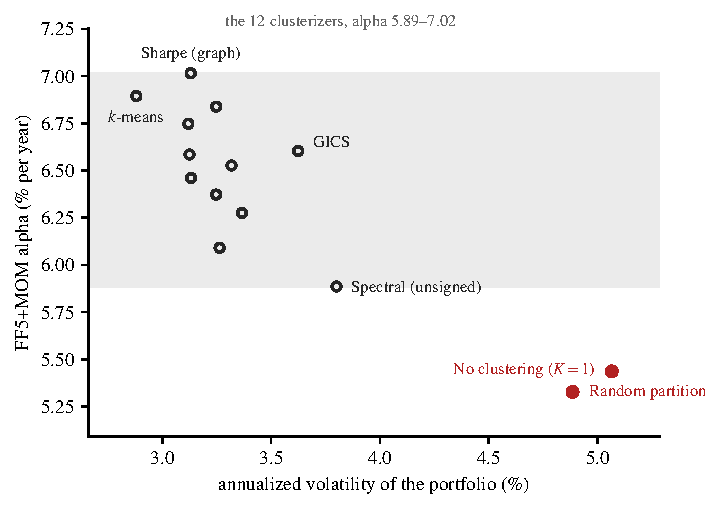
\includegraphics[width=\linewidth]{fig_alpha_vol}
\caption{Alpha against volatility in the trained component. This figure plots
each trained portfolio's annualized alpha against its annualized volatility over the
$6{,}913$-day sample (July 1997 to December 2024). As in \tabref{tab:moments},
alphas are against FF5+MOM with Newey--West(21) standard errors on the
seed-averaged payoff, and volatilities are computed per head seed and averaged over the five head seeds. The shaded band
covers the range of the 12 clusterizers' alphas. Four clusterizers are labeled. Among the 12 clusterizers, $k$-means on
returns has the lowest volatility. Sharpe (graph) has the highest alpha. \textsc{gics} has the second-highest volatility and a mid-band alpha. Unsigned spectral clustering has the highest volatility and the lowest alpha. The eight unlabeled circles are the remaining clusterizers, whose
coordinates are listed in the replication package. The two controls are red.}
\label{fig:alpha_vol}
\end{figure}



%%  THREE PARAGRAPHS.
%%  P1  the numbers, WITHIN each layer, both controls.
%%        rule-based   methods 4.704-6.932 %/yr   k1 8.850   random 8.433
%%        trained      methods 2.741-3.619        k1 4.773   random 4.995
%%      close on: training barely narrows it -- vs k1 39.9 -> 33.9 %,
%%      vs random 36.9 -> 36.8 % (i.e. not at all).
%%  P2  the supports do not overlap. Best control run 1.5489 < worst
%%      method run 1.7739 across 43 gate-passing runs. This is stronger
%%      than any comparison of means; give it its own sentence.
%%  P3  the cut does not depend on WHICH rule produces it (2.741-3.619
%%      all far from 4.773) -> the hedge is a property of clustering as
%%      such, not of a well-chosen clustering. Forward-point to §5.
%%
%%  ⛔ no cross-layer level comparison (windows 5 vs 30, gross 2 vs 1)
%%  ⛔ no percentage without naming its control
%%  ⛔ "forces / imposes group neutrality" -- refuted, see §4.3


Clustering also raises alpha. We call the percentage by which the clusterizers' alpha exceeds the alpha of a control the alpha advantage. As with the volatility reduction, the size of the alpha advantage depends on which trading component trades the signal. In the rule-based component, both controls earn less alpha than each of the 12 clusterizers. The alphas of the 12 clusterizers range from $4.03\%$ to $4.40\%$ per year. The alpha is $3.63\%$ for the $\K=1$ control and $3.72\%$ for the random control. In relative terms, the mean rule-based alpha of the 12 clusterizers is $15.6\%$ higher than that of the $\K=1$ control and $13.1\%$ higher than that of the random control. Because the fixed rule has no fitted parameters and the rule-based configurations differ only in the signal they receive, the extra alpha must come from the group-demeaned residuals that the partition defines (\eqnref{eq:relsig}).

Measured against FF5+MOM, the six factors of \tabref{tab:moments}, the alpha advantage over both controls is larger in the trained component than in the rule-based component. The advantage widens much more over the random control than over the $\K=1$ control. Against the $\K=1$ control, the six-factor advantage rises from $15.6\%$ in the rule-based component to $20.0\%$ in the trained component. Against the random control, it rises from $13.1\%$ to $22.5\%$. A wrong partition therefore has a larger disadvantage in the trained component than in the rule-based component, in the sense that the random control falls further behind the clusterizers in alpha (\secref{sec:head}). However, when a short-term reversal factor is added, the rule-based advantage exceeds the trained advantage (\secref{sec:spanning}).

Clusterizer by clusterizer, the advantage over the random control is also more robust than the advantage over the $\K=1$ control. Both advantages are positive for all 12 clusterizers. We also compute the advantage separately for each head seed, so that it has a dispersion across a clusterizer's five head seeds. The advantage over the random control exceeds twice this dispersion for seven of the 12 clusterizers. The advantage over the $\K=1$ control does so for four of the 12. The count of four does not change when we use the dispersion pooled over the 12 clusterizers instead of each clusterizer's own dispersion, although the two dispersions do not select the same four clusterizers.
%%  RECORD, not an open item. On the old panel this paragraph read the
%%  other way: the advantage over K=1 was reported to fall by more than
%%  half while the advantage over random held. On v3 both rise. Two
%%  supporting claims were carried over only after recomputation. The
%%  era concentration reversed, and tab:signal's note now states the
%%  later era as the larger one. The per-rule count was recomputed on
%%  v3 and is now in the text above: 5 of 12 against K=1, 12 of 12
%%  against random, positive at all twelve arms against both. Source:
%%  server_package/e2e_plan/perrule_count_v3.csv.

In the trained component, the random control earns less alpha than the $\K=1$ control ($5.33$ against $5.44$). One plausible explanation for this gap is the noise that random groups add to the $\K=1$ signal. Demeaning within a random group subtracts the average market residual of roughly 16 unrelated stocks. Under the random partition, the group-demeaned residual is therefore the $\K=1$ group-demeaned residual perturbed by a term that contains little systematic information about comovement. As a result, the trading head receives a noisier version of the signal that it receives under $\K=1$.


%%  THE PIVOT OF THE SECTION. Two controls part ways under training.
%%  P1  rule-based: k1 6.066 and random 6.314 are the LOWEST alphas of
%%      the twenty-one; methods 6.805-8.729, mean 7.464 (+23.0 % vs k1,
%%      +18.2 % vs random).
%%  P2  trained: advantage over k1 halves to +14.0 % (calendar-aligned
%%      FF5+MOM), outside head-seed noise for 11 of 12 -- BUT ⛔ it is
%%      entirely pre-2009 (2009-24: methods mean 2.87 vs k1 2.90, 7 of 12
%%      BELOW k1). Never claim a modern-era edge over K=1.
%%  P3  against random the advantage does NOT shrink: +33 %, 12 of 12
%%      outside noise. THE SENTENCE THE SECTION EXISTS FOR:
%%        a trained model substitutes for a clustering it was never given,
%%        and does not repair one it was given wrongly.
%%  P4  (was the old second reading) at the rule-based layer BOTH moments
%%      improve, so "alpha is nearly flat" is a trained-layer statement.

\subsection{Variance Removed by Group Demeaning}
\label{sec:mechanism}

Under a real partition, demeaning within groups removes $11\%$ to $26\%$ of the cross-sectional variance of the day's market residuals. Under a random partition, the variance share equals the degrees-of-freedom floor. We measure the variance share directly. For each clusterizer and each control, we take each day's market residuals (\secref{sec:resid}) and subtract from each stock the mean market residual of its group, as in \eqnref{eq:relsig}. The variance share is the share of the cross-sectional variance that this subtraction removes. For the 12 clusterizers, the variance share ranges from $10.8\%$ for the \textsc{gics} sector taxonomy to $26.4\%$ for $k$-means on returns. The value for $k$-means on returns counts its singleton groups. Each singleton group removes all of the variance of its one member (\appref{app:lensrobust}). The variance shares of the other 10 clusterizers range from $17.0\%$ to $19.1\%$, within about two percentage points of one another. These clusterizers nevertheless disagree widely on the partition (\secref{sec:pseed}).

For the $\K=1$ control, the variance share is zero by construction, because its single group's mean \emph{is} the cross-sectional mean, around which the variance is already measured. The group-demeaned residual of the $\K=1$ control therefore has the same cross-sectional variance as the market residual.

The random control measures the part of the variance share that is unrelated to structure. Subtracting a group mean removes some variance even when the groups are meaningless. With $\K$ random groups over $\N_t$ stocks, the expected variance share is $(\K-1)/(\N_t-1)$, the degrees-of-freedom floor. At $\K=30$, the floor is $5.88\%$. We compute it on the $494.3$ stocks that the rule-based portfolio trades on an average day. The random control's variance share is $5.93\%$, so the floor accounts for everything it removes. Consistent with this result, the random control's portfolio remains one of the two most volatile of the 14 portfolios. Removing variance that does not come from comovement therefore does little to lower the volatility of the portfolio.

The removed comovement explains the lower volatility of the portfolio. With that comovement removed, the positions that the head builds on the signal comove less. In particular, in the spanning regressions of \secref{sec:spanning}, the 12 clusterizers' trained portfolios have $42\%$ less market beta than the $\K=1$ control and $35\%$ less than the random control. Moreover, from no clustering to a random partition to a real partition, the variance share rises and portfolio volatility falls in both trading components (\secref{sec:hedge}). Similarly, when we degrade a partition step by step toward a random partition, the variance share falls toward the degrees-of-freedom floor and portfolio volatility rises at every step (\appref{app:dose}).

Balance within groups could also lower the volatility of the portfolio. The group-demeaned residuals sum to zero within each group, so the positions of the portfolio could inherit that balance. However, in our portfolios, balance contributes little to the volatility reduction. A typical group's longs and shorts are out of balance by $16\%$ to $23\%$ of the group's total position. This imbalance is $71\%$ to $85\%$ of the imbalance that random signs on the same weights would produce. The exception is \textsc{gics}, whose imbalance exceeds its own random level.

\subsection{Decomposing the Sharpe Gap}
\label{sec:split}

Most of the Sharpe gap between the clusterizers' portfolios and either control arises through volatility. Because the log Sharpe ratio is the log mean minus the log volatility, the log-Sharpe gap between the clusterizers' portfolios and the control portfolios splits exactly into the mean part and the volatility part,
\begin{equation}\label{eq:split}
\log \mathrm{SR}_g-\log \mathrm{SR}_c=(\log\mu_g-\log\mu_c)-(\log\sigma_g-\log\sigma_c).
\end{equation}
In \eqnref{eq:split}, the clusterizers' mean and volatility are the averages over the clusterizers of their annualized means and volatilities, and the mean and volatility of the control are its own. In the trained component, the volatility part is $82.0\%$ of the gap to the $\K=1$ control (\tabref{tab:split}). We call the volatility part divided by the gap the volatility share of the gap. Across the four cells of the table, the volatility share ranges from $75\%$ to $83\%$ and is largest in the rule-based component against the random control. Because this split uses mean returns, any return that the controls earn from factor exposure enters their means. With FF5+MOM alphas in place of the mean returns, the volatility reduction still accounts for most of the Sharpe gap (notes to \tabref{tab:split}).

\begin{table}[tb]
\centering
\caption{Mean and volatility parts of the log-Sharpe gap to each control}
\label{tab:split}
\begin{threeparttable}
\small
\begin{tabular}{@{}llcccc@{}}
\toprule
Trading component & Control & Gap & Mean part & Volatility part & Volatility share \\
\midrule
Rule-based & $\K=1$  & $0.667$ & $0.124$ & $0.543$ & $81.4\%$ \\
Rule-based & Random  & $0.590$ & $0.100$ & $0.490$ & $83.0\%$ \\
Trained & $\K=1$ & $0.533$ & $0.096$ & $0.437$ & $82.0\%$ \\
Trained & Random & $0.532$ & $0.131$ & $0.401$ & $75.4\%$ \\
\bottomrule
\end{tabular}
\begin{tablenotes}[flushleft]\footnotesize
\item \emph{Notes.} This table reports the log-Sharpe gap between the 12 clusterizers and each control and its split into a mean part and a volatility part, by trading component. All configurations use the common 60-day estimation window and are measured on the $6{,}913$-day sample of \secref{sec:panel} (July 1997 to December 2024). For the clusterizers, $\mu$ and $\sigma$ are the means over the 12 clusterizers of the annualized mean and of the annualized volatility. Each control uses its own mean and volatility. Gap is the left side of \eqnref{eq:split}. The mean part is $\log\mu_g-\log\mu_c$, the volatility part is $\log\sigma_c-\log\sigma_g$, and the volatility share is the volatility part divided by the gap. In the trained cells, $\mu$ and $\sigma$ are computed per head seed and averaged over the five head seeds. Averaging the payoff series over head seeds before computing $\mu$ and $\sigma$ instead gives a volatility share of $80.2\%$ against the $\K=1$ control and $71.6\%$ against the random control. The rule-based component has no head seed. Clusterizer by clusterizer, in the trained cells the volatility share is lowest for Sharpe (graph) against the $\K=1$ control and for \textsc{gics} against the random control. The lower of these two values is $67.8\%$. Every other clusterizer stays at or above $69\%$ in every cell. Replacing the means with calendar-aligned alphas in the trained cells gives a mean part of $0.182$ against the $\K=1$ control and $0.203$ against the random control. The mean part is then $29.4\%$ of the recomputed gap against the $\K=1$ control and $33.6\%$ against the random control.
\end{tablenotes}
\end{threeparttable}
\end{table}

%%  P1  THE LADDER. The signal is residualized twice -- once against the
%%      market (eq:residual), once against the peer group (eq:relsig).
%%      How much the second step removes:
%%        k1        2.6 % mean / 1.2 % median   (right-skewed, quote both)
%%        random    5.93 %  == the structureless floor (K-1)/(N-1)=5.95 %
%%        methods   17.5-20.2 %
%%        GICS      16.6 %, about a point BELOW the band
%%      So k1's signal is effectively once-residualized. Random's removal
%%      is ARITHMETIC, not structure -- and its book is the most volatile
%%      in the field: demeaning within meaningless groups spends breadth
%%      without hedging anything.
%%      ⭑ the floor is DERIVABLE: a rank-K projection on an already
%%        centred cross-section removes (K-1)/(N-1) in expectation with
%%        no structure. 29/489 = 5.93 %. State it as arithmetic.
%%  P2  TRANSMISSION, in its DEMOTED form. We tested whether the trained
%%      book inherits within-cluster dollar neutrality. IT DOES NOT --
%%      median cluster tilt is 16-19 % of cluster gross, at 0.97 of a
%%      sign-randomization null for random and 0.84 for a real clustering.
%%      The hedge runs through the correlation structure of the bets a
%%      demeaned signal induces; corroboration is the halved market beta
%%      (0.030-0.050 vs k1 0.071, random 0.105).
%%      ⛔ Only an ORDINAL map across the three coarse rungs. There is no
%%        dose-response inside the method band (spectral removes
%%        mid-band yet is nearly the highest-vol data-driven arm).
%%      ⛔ "imposes group neutrality" in any form.

%%  ── tab:dispersion RETIRED 2026-08-16 ──────────────────────────────
%%  Its c.v. columns are the OLD cross-configuration statistic that the
%%  controls created (methods-only ratio 0.96). Replaced by tab:hedge
%%  (§4.1) and a signal table to come (§4.2). Source kept below.
%% \begin{table}[tb]
%% \centering
%% \caption{Dispersion of the two moments across configurations, at both
%% trading layers}
%% \label{tab:dispersion}
%% \begin{threeparttable}
%% \begin{tabular}{@{}lcccccc@{}}
%% \toprule
%% & \multicolumn{2}{c}{Annualized alpha (\%)}
%% & \multicolumn{2}{c}{Annualized volatility (\%)} & \\
%% \cmidrule(lr){2-3}\cmidrule(lr){4-5}
%% Trading layer & range & c.v. & range & c.v. & ratio \\
%% \midrule
%% Rule-based & $6.066$--$8.729$ & $7.9\%$ & $4.704$--$8.850$ & $18.2\%$ & $2.30$ \\
%% Trained    & $6.085$--$7.689$ & $5.5\%$ & $2.434$--$4.584$ & $18.8\%$ & $3.42$ \\
%% \bottomrule
%% \end{tabular}
%% \begin{tablenotes}[flushleft]\small
%% \item \emph{Notes.} Alpha is against the Fama--French five factors plus
%% momentum with Newey--West(21) standard errors, 6,941 out-of-sample days.
%% The coefficient of variation is the cross-configuration standard
%% deviation divided by the mean; the last column is the volatility
%% coefficient divided by the alpha coefficient. The trained layer covers
%% the nineteen configurations listed in the appendix, on the
%% seed-averaged Sharpe convention; the rule-based layer covers the
%% twenty-one partitions for which a rule-based book exists. The two layers
%% use different signal windows and gross-exposure conventions, so only the
%% \emph{within-layer} dispersion is comparable across them.
%% \end{tablenotes}
%% \end{threeparttable}
%% \end{table}

%% RETIRED 2026-08-18 (was orphaned; old arm set):
%% \begin{table}[tb]
%% \centering
%% \caption{Exact decomposition of the cross-configuration variance of the
%% log Sharpe ratio}
%% \label{tab:vardecomp}
%% \begin{threeparttable}
%% \begin{tabular}{@{}lcc@{}}
%% \toprule
%% & Return channel & Volatility channel \\
%% \midrule
%% Share of $\operatorname{var}(\log \mathrm{SR})$ & $13.51\%$ & $86.49\%$ \\
%% \addlinespace
%% $\operatorname{corr}(\log \mu, \log \sigma)$, nineteen configurations
%%   & \multicolumn{2}{c}{$-0.1768$} \\
%% $\operatorname{corr}(\log \mu, \log \sigma)$, twelve methods only
%%   & \multicolumn{2}{c}{$+0.4511$} \\
%% \bottomrule
%% \end{tabular}
%% \begin{tablenotes}[flushleft]\small
%% \item \emph{Notes.} Since $\log \mathrm{SR} = \log\mu - \log\sigma$,
%% $\operatorname{var}(\log \mathrm{SR}) = \operatorname{cov}(\log \mathrm{SR},\log\mu)
%% - \operatorname{cov}(\log \mathrm{SR},\log\sigma)$ identically; the
%% residual is $4\times10^{-16}$. The shares pair $\mu$ with the spanning
%% alpha. Pairing it with the realized mean return gives $18.09\%$ and
%% $81.91\%$. Across the five configuration sets examined the volatility
%% share ranges from $72\%$ to $86\%$. Nineteen configurations; the
%% twelve-method row excludes both controls and the five window twins.
%% \end{tablenotes}
%% \end{threeparttable}
%% \end{table}

%%---------------------------------------------------------------------
%%  §4.2 DRAFT, 2026-08-15. Yours to edit. RE-APPLIED after an editor
%%  save overwrote it; if it disappears again, it is a concurrent-write
%%  collision and not a deletion.
%%
%%  WHAT THE THREE PARAGRAPHS DO:
%%   1  states the alternative explanation and the test, IN THAT ORDER. A
%%      test whose result is announced first reads as a search for
%%      confirmation. Note it does not say "a reader might object" -- the
%%      Sharpe objective's interest in the second moment is a fact about
%%      the objective, stated as one.
%%   2  the result, with the caveat IN THE SAME SENTENCE as the comparison
%%      it constrains. ⛔ Not in a footnote, not a paragraph later.
%%   3  the second reading. ⛔ Do not omit and do not soften: at the
%%      rule-based layer clustering improves BOTH moments, so "alpha is
%%      flat" is trained-layer only.
%%
%%  ⛔ NO CROSS-LAYER ALPHA LEVEL DIFFERENCE ANYWHERE. There is a tempting
%%     pattern in the per-configuration changes -- the model appears to
%%     lift weak clusterizations and lower strong ones -- and it is confounded
%%     by the 5-day against 30-day signal window.
%%
%%  ⚠ NUMBERS UNDER AUDIT: 2.30, 3.42, 18.2, 18.8, 6.066 / 6.314 / 8.729.
%%    Source scripts/naive_spanning.csv, NUMBERS.md N12.5. The paragraph
%%    structure survives any correction; "present before the model and
%%    larger after it" needs only 1 < 2.30 < 3.42, a wide margin.
%%
%%  ⚠ N22 BITES LESS HERE THAN IN §4.1. Both layers are measured on one
%%    partition draw, but the layer CONTRAST is within-draw, so a draw
%%    effect would have to hit one layer and not the other to overturn
%%    it. §4.1's c.v. levels are exposed to it directly; this ratio is not.
%%---------------------------------------------------------------------

%%---------------------------------------------------------------------
%%  §4.1 DRAFT, 2026-08-15. Yours to edit.
%%
%%  WHAT THE THREE PARAGRAPHS DO:
%%   1  the contrast, read off the table. The ranges are given as BAND
%%      WIDTHS, not endpoints, because the endpoints (6.085, 7.689, ...)
%%      are all in the audit and two of them are disputed -- NUMBERS.md N2
%%      puts the alpha lower bound at 6.48 against the table's 6.085. Band
%%      widths and the c.v.s survive either resolution; endpoints do not.
%%      Put the endpoints back in prose only if you want them repeated
%%      from the table, which is usually dead weight.
%%   2  the ANOVA, and the sentence people get wrong. Leads with "the
%%      alphas are not equal" so no reader can take the section for an
%%      equality claim.
%%   3  the figure.
%%
%%  ⛔ TWO NORMALIZATIONS, NOT THREE. An earlier note here claimed the
%%     §3.6 ratios (12-23 against 0.8-2.1) were a third measure agreeing
%%     at "about three". They are not -- that comparison is nearer ten,
%%     because §3.6 divides by ESTIMATION error, which at T = 6,941 is
%%     tiny for a volatility. It answers a different question and its
%%     figures are not on the same scale. Only the c.v. and the
%%     between/within ratio belong in the "both give about three"
%%     sentence.
%%
%%  ⚠ THE c.v. CONCESSION IS DELIBERATE. Saying that a coefficient of
%%     variation flatters the smaller quantity, and that volatility is
%%     the smaller quantity here, gives away a real weakness of the first
%%     measure. It is not defensiveness -- it is the reason the second
%%     measure exists, and stating it is why the paragraph needs two
%%     normalizations at all rather than looking like it is piling them up.
%%
%%  ⚠ THE TWO \PH{ratio} SLOTS are the between/within figures and they
%%    are IN CONFLICT: this file's header says 3.03 (vol) against 1.12
%%    (alpha); NUMBERS.md N3.2 says 2.744 against 1.112. Left as
%%    placeholders on purpose -- the prose says "roughly three times",
%%    which is true on either. Fill when the audit returns.
%%
%%  ⛔ NOT WRITTEN, deliberately: any sentence explaining why a
%%     coefficient of variation is the right comparison, or why an ANOVA
%%     uses the seed replicates. A referee at this venue knows both.
%%  ⛔ AND no sentence disclaiming that this is not a stability claim.
%%     It isn't one; say nothing.
%%
%%  ⚠ \PH{} DOES NOT LINE-BREAK -- it wraps its argument in \text{}, so a
%%    placeholder longer than a few words overflows the line. Use \PH for
%%    a missing NUMBER and \TODO for a missing paragraph or figure.
%%---------------------------------------------------------------------

%%---------------------------------------------------------------------
%%  THE SCOPE PARAGRAPH, 2026-08-15. Read before touching the opening.
%%
%%  ⛔ A \TODO RENDERS. It is reader-facing text in red, even when the
%%     reader is a coauthor, so it is a QUESTION and never an argument.
%%     The first draft of the title TODO ran 120 words weighing both
%%     sides, which reads in the PDF as exactly the hand-wringing this
%%     section is trying not to do. Reasoning goes in %%; the question
%%     goes in \TODO. Same rule as the framing and register ones.
%%
%%  THE TITLE QUESTION, in full, since the \TODO now only asks it:
%%    "not its return" asserts an absence. §3.6 establishes only that the
%%    design cannot SEE a return effect, and not seeing one is not the
%%    same as its absence. Two ways out -- soften the title, or keep it
%%    as a compression and let the scope sentence carry the precision,
%%    which is what is drafted. Either is defensible; the drafted one
%%    keeps a claim-style title consistent with the other sections.
%%
%%  WHAT THE EVIDENCE SUPPORTS, and it is less than the title:
%%    STANDS  the variance decomposition, 13.51 / 86.49. It is an
%%            IDENTITY on the observed numbers (residual 4e-16), needs no
%%            inference, and is untouched by any resolution limit. This is
%%            the hardest thing in the section -- lead the evidence on it.
%%    STANDS  volatility differences are 12-23x their measurement error;
%%            mean-return differences are 0.8-2.1x theirs (§4).
%%    STANDS  "a smaller variance without a COMMENSURATE change in the
%%            mean" -- commensurate means proportionate, and that is
%%            defensible. The author's own wording was already correct.
%%    FAILS   "clustering does not affect return". Absence of evidence is
%%            not evidence of absence, and §4 says only that we cannot
%%            see it.
%%
%%  ⚠ THE APPARENT CONTRADICTION A REFEREE WILL FIND, now handled in the
%%    paragraph above but keep it handled: §5.1's ANOVA REJECTS equal
%%    alphas (F = 3.775, p = 2.5e-4) while §4 says return differences are
%%    at the resolution limit. Both are true; the denominators differ.
%%    The ANOVA asks whether arms differ by more than HEAD-TRAINING noise;
%%    §4 asks whether they differ by more than the error in estimating a
%%    mean from 6,941 days. Never print one without the other nearby.
%%
%%  ⚠ AND §4's license has a dependency: it rests on the last era's ratio
%%    being 0.8, i.e. BELOW one. If the audit of 2026-08-15 moves that
%%    figure above one, "below it" must go and this framing needs
%%    revisiting -- "cannot see" would become "can see, and it is small",
%%    which is a different and weaker claim.
%%
%%  ⚠ NEW 2026-08-15, AND THE AUDIT WILL NOT CATCH IT. Every dispersion
%%    figure in this section is measured on ONE partition draw. Each
%%    method's partition was generated once, at generation seed 42, and
%%    the three runs behind each c.v. vary only the head initialization
%%    (§3.5). CORRECTIONS.md N22 now measures what a different partition
%%    draw does: on the deterministic naive layer the partition-seed s.d.
%%    is 0.0693 for kmeans_ret against a head-seed s.d. of 0.0152, and the
%%    TOP of the ranking flips between draws.
%%      What this does and does not threaten:
%%      - the ASYMMETRY is very likely robust. It is a contrast between
%%        two columns measured on the same draw, so a draw effect has to
%%        hit one moment and not the other to overturn it.
%%      - the VALUES are one draw. 5.5% and 18.8% each carry an unmeasured
%%        component, and the ratio 3.42 with them.
%%    ⛔ Do not write "the c.v. of alpha is 5.5%" as though it were a
%%       population quantity. Either attach the draw, or wait: the head
%%       runs for three partition seeds are queued and land within a day.
%%    ⛔ And do not extend §4.1's ANOVA to partition seeds. The design is
%%       an L through the 3x3 grid -- both marginals, no interaction --
%%       so an ANOVA assuming additivity would be estimating a term that
%%       was never sampled (N22 caveat (c)).
%%
%%  ⚠ UNRESOLVED NUMBER CONFLICT, for the audit: this file's header says
%%    between/within sd 3.03 (vol) against 1.12 (alpha); NUMBERS.md N3.2
%%    says 2.744 against 1.112. Do not print either until settled.
%%---------------------------------------------------------------------

%%---------------------------------------------------------------------
%%  TABLES, READY TO USE. Every value recomputed from source 2026-08-14
%%  (spanning.csv restricted to the nineteen; the rule-based layer from
%%  naive_pnl_sigw5.pkl regressed on FF5+MOM with Newey-West(21) using
%%  the repository's own load_ff and nw_ols). Write the prose around
%%  them; do not retype the numbers.
%%---------------------------------------------------------------------

%%---------------------------------------------------------------------
%%
%%  5.1  THE DISPERSION CONTRAST                        ~700 words
%%
%%  P1  (~120 w)  The setup.
%%      FIRST SENTENCE: state that the panel, the residualization, the
%%        trading model, the target number of groups and the seeds are
%%        common to every configuration and only the partition changes.
%%        Point back to \secref{sec:design}.
%%      MIDDLE: therefore whatever separates the configurations is
%%        attributable to the clusterizer.
%%      LAST SENTENCE: the question is not how large that separation is
%%        but WHERE IT LANDS. Name the answer -- the second moment --
%%        and say the section establishes it in three steps.
%%
%%  P2  (~250 w)  The contrast.       -> \tabref{tab:dispersion}, trained row
%%      FIRST SENTENCE: the two moments do not spread alike.
%%      MIDDLE: alpha 6.085-7.689 %/yr against volatility 2.434-4.584 %;
%%        coefficients of variation 5.5 % and 18.8 %; ratio 3.42.
%%      THEN THE ANOVA, and this is the sentence people get wrong.
%%        The alphas are NOT equal -- a one-way ANOVA on the seed
%%        replicates rejects equality at F = 3.775, p = 2.546e-4. What is
%%        true is a MAGNITUDE contrast: between-configuration over
%%        within-configuration standard deviation is 3.03 for volatility
%%        and 1.12 for alpha.
%%      MODEL SENTENCE, adapt it, do not copy it:
%%        "The alphas are not identical -- an ANOVA on the seed
%%         replicates rejects that -- but they are close in a way the
%%         volatilities are not: relative to the noise in its own
%%         measurement, the spread in volatility is nearly three times
%%         the spread in alpha."
%%      LAST SENTENCE: hand off to the figure.
%%      ⛔ Never write "every clustering earns the same alpha".
%%
%%  P3  (~150 w)  The figure.         -> \figref{fig:alpha_vol}
%%      Say what a reader sees: one point per configuration, alpha on one
%%      axis and volatility on the other, the cloud narrow in one
%%      direction and wide in the other. Name where the two controls sit.
%%      Do not re-state the numbers already in P2.
%%
%%---------------------------------------------------------------------
%%
%%  5.2  THE SAME CONTRAST ONE LAYER DOWN               ~800 words
%%       *** WRITE THIS FIRST. It is the section's real content. ***
%%
%%  P4  (~150 w)  Why this test exists.
%%      FIRST SENTENCE: state the alternative explanation you are about
%%        to rule out -- that the asymmetry is a property of the trained
%%        model rather than of the clustering.
%%      MIDDLE: the test. Remove the model. If the asymmetry is the
%%        model's, it should go with it.
%%      LAST SENTENCE: say what the rule-based book is, in one clause
%%        (no fitted parameter anywhere), and point at \secref{sec:design}.
%%      ⭑ State the test BEFORE the result. A test whose result is
%%        announced first reads as a search for confirmation.
%%
%%  P5  (~250 w)  The result.         -> \tabref{tab:dispersion}, both rows
%%      FIRST SENTENCE: the asymmetry survives.
%%      MIDDLE: ratio 2.30 at the rule-based layer against 3.42 at the
%%        trained one; the volatility coefficient barely moves between
%%        layers (18.2 % against 18.8 %).
%%      ⚠ THE CAVEAT GOES IN THIS PARAGRAPH, IN THE SAME SENTENCE AS THE
%%        COMPARISON IT CONSTRAINS -- not in a footnote, not in the table
%%        note, not two paragraphs later. The two layers run a five-day
%%        and a thirty-day signal window at different gross-exposure
%%        conventions, so only the WITHIN-layer dispersion is comparable
%%        and no cross-layer difference in level may be read off.
%%      MODEL SENTENCE:
%%        "Because the two books run different signal windows at
%%         different gross conventions, the comparison that follows is
%%         between the two layers' internal dispersions and not between
%%         their levels."
%%      LAST SENTENCE: so the asymmetry belongs to the clustering.
%%
%%  P6  (~250 w)  THE SECOND READING. Do not omit it. Do not soften it.
%%      FIRST SENTENCE: the flatness of alpha does not survive the change
%%        of layer, and that is a separate fact from the asymmetry.
%%      MIDDLE: at the rule-based layer the two controls hold the two
%%        LOWEST alphas of the twenty-one -- no clustering 6.066 and random
%%        clustering 6.314, against 8.729 for complete linkage. So at that
%%        layer clustering improves BOTH moments, unequally.
%%      LAST SENTENCE, and it is the section's most important sentence:
%%        the asymmetry is a statement about both layers; the FLATNESS of
%%        alpha is a statement about the trained one. Every later use of
%%        the flat-alpha result carries that qualifier.
%%      ⛔ Do not print any cross-layer alpha LEVEL difference. There is a
%%        tempting pattern in the per-configuration changes -- the model
%%        appears to lift weak clusterizations and lower strong ones -- and it
%%        is confounded by the signal window. Say in one clause that it
%%        is not reported and why.
%%
%%---------------------------------------------------------------------
%%
%%  5.3  THE EXACT DECOMPOSITION                        ~700 words
%%
%%  P7  (~150 w)  The algebra.        -> \tabref{tab:vardecomp}
%%      Two displayed lines. log SR = log mu - log sigma, therefore
%%      var(log SR) = cov(log SR, log mu) - cov(log SR, log sigma),
%%      additively and with no residual term. Say that this is an
%%      identity, not an approximation, and that the measured residual is
%%      4e-16.
%%      ⭑ Say why an identity is worth printing: it removes the
%%        arbitrariness of any weighting one might otherwise choose.
%%
%%  P8  (~200 w)  The result.
%%      13.51 % of the cross-configuration variance on the return side,
%%      86.49 % on the volatility side. Then the two robustness facts:
%%      pairing mu with the realized mean instead of the alpha gives
%%      18.09/81.91, and across the five configuration sets examined the
%%      volatility share runs 72-86 %. State the pairing you are using in
%%      the sentence, not only in the table note.
%%
%%  P9  (~200 w)  THE REFUSAL.
%%      FIRST SENTENCE: one quantity in the table is not robust and is
%%        therefore not used.
%%      MIDDLE: corr(log mu, log sigma) is -0.1768 over the nineteen and
%%        +0.4511 over the twelve methods alone. The sign is a property of
%%        the configuration set, not of the data.
%%      LAST SENTENCE: therefore no claim is made about whether the
%%        variance reduction is paid for in return, in either direction.
%%      ⭑ Write this as a result about what the design can and cannot
%%        identify, not as an apology.
%%
%%  P10 (~150 w, optional but recommended)  A second refusal.
%%      The correlation between the Sharpe ratio and inverse volatility is
%%      0.9478 and is not reported as evidence: since SR = mu/sigma the
%%      statistic is near-arithmetic, and a permutation null that destroys
%%      every economic link already has mean 0.93-0.94. One short
%%      paragraph. A referee who was going to compute it themselves stops
%%      here.
%%
%%=====================================================================

%%=====================================================================
%%  §4.4  merged from 06_trading_model.tex on 2026-08-27 (user request)
%%=====================================================================
%%=====================================================================
%%  §6  THE TRADING MODEL AS THE MIRROR          target 3 pp.
%%
%%  7.1  THE MODEL, at a level an econometrician can evaluate. Inputs,
%%       what is learned, the objective, the walk-forward protocol:
%%       training and validation window lengths, retraining frequency,
%%       epoch budget, early-stopping rule. ⚠ The generated draft omitted
%%       the protocol entirely and a referee flagged it -- "no
%%       econometrics referee will pass a paper that omits this".
%%       Read it off an executed run's working copy.
%%
%%  7.2  THE RESULT. At MATCHED gross exposure, over 21 configurations:
%%         alpha  +3.2632 pp/yr,  21 of 21 positive
%%         volatility ratio median 1.0439,  18 of 21 ABOVE 1
%%       The model raises the first moment and leaves the second where it
%%       was -- the mirror image of §5.
%%       ⚠ CAVEAT THAT MUST BE PRINTED: once gross is aligned the moment
%%       split is an ALGEBRAIC RE-EXPRESSION of the Sharpe comparison, not
%%       independent evidence. What makes it non-trivial is the empirical
%%       fact that the rule-based book at gross 1.0 already sits at the
%%       trained book's volatility. Say exactly that.
%%       The alignment itself is an exact 0.5 rescale, not a fit: the
%%       rule-based book is +1/n_long and -1/n_short by construction and
%%       the trained book measures L1 norm 1.0 within 2 fp32 ulps.
%%
%%  7.3  THE REORDERING, and the methodological consequence. A method
%%       placed 8th under the rule-based book rises to 3rd under the
%%       learned one; six of eighteen arms move three or more places;
%%       between-layer Spearman +0.8390 (p = 1.35e-5).
%%       ⚠ NAME THE ARM SET -- "sixth to second" is a twelve-arm
%%       statement and "eighth to third" an eighteen-arm one. Both true.
%%       ⛔ Do NOT write "the ordering does not survive the change of
%%          trading model". At +0.84 it largely DOES. The claim is that
%%          individual positions move enough that a downstream Sharpe
%%          ratio cannot rank an upstream representation.
%%
%%  7.4  THE LAYER REVERSAL -- new, and it links §6 to §7 causally.
%%         rule-based:  random 0.8123  >  no clustering 0.7504
%%         trained:     no clustering 1.4107  >  random 1.2662
%%       A wrong clustering becomes costly only once a model is trained on
%%       it. The head is what makes a bad partition expensive.
%%
%%  FIGURES: fig_deep_vs_naive or fig_rank_shift if lifted from the
%%  comprehensive draft's figure set.
%%
%%  ⛔ No individual head-lift point value. It is a bound: +0.74 to +1.50.
%%     The naive comparator uses a 5-day signal window and the head 30;
%%     matching them does not close the gap, it doubles it.
%%=====================================================================
\subsection{The Contribution of the Trading Head}
\label{sec:head}

In Sections \ref{sec:hedge} to \ref{sec:split}, we compared partitions within each trading component. We now compare the two trading components on the same partition and ask what the neural trading head contributes to the performance.





\tabref{tab:head_adds} compares the rule-based and the trained portfolio of each clusterizer and each control.  The head raises alpha in every portfolio, including the two control portfolios. Although the head is trained on an objective that divides by the standard deviation, it also raises volatility in every portfolio, by $9\%$ to $24\%$. In proportion, this rise is smaller than the rise in alpha.

\begin{table}[tb]
\centering
\caption{Alpha and volatility in the rule-based and trained components, and the change between them}
\label{tab:head_adds}
\begin{threeparttable}
\small
\begin{tabular}{@{}lcccccc@{}}
\toprule
& \multicolumn{3}{c}{Alpha (\%/yr)} & \multicolumn{3}{c}{Volatility (\%/yr)} \\
\cmidrule(lr){2-4}\cmidrule(lr){5-7}
& Rule-based & Trained & Gain & Rule-based & Trained & Ratio \\
\midrule
12 clusterizers & $4.03$--$4.40$ & $5.89$--$7.02$ & $+1.56$ to $+2.94$ & $2.38$--$3.09$ & $2.88$--$3.80$ & $1.17$--$1.24$ \\
$\K=1$ & $3.63$ & $5.44$ & $+1.80$ & $4.65$ & $5.07$ & $1.09$ \\
Random & $3.72$ & $5.33$ & $+1.61$ & $4.41$ & $4.89$ & $1.11$ \\
\bottomrule
\end{tabular}
\begin{tablenotes}[flushleft]\small
\item \emph{Notes.} This table reports the alpha and volatility of each clusterizer and each control in both trading components, and the change from the rule-based to the trained component. All 14 configurations of each trading component use the common 60-day estimation window and are measured on the $6{,}913$-day sample of \secref{sec:panel} (July 1997 to December 2024). Alphas are against FF5+MOM with Newey--West(21) standard errors, with each trading component joined to the factor file on its own realization calendar (\appref{app:calendar}). Rule-based cells repeat the rule-based entries of \tabref{tab:moments}. Gain is the trained alpha minus the rule-based alpha, in percentage points. Ratio is the trained volatility divided by the rule-based volatility. Both are computed separately for each clusterizer and control on unrounded values. The 12-clusterizer row is therefore the range of the per-clusterizer values, not the difference or ratio of the printed ranges. As in \tabref{tab:moments}, volatility columns are computed per head seed and averaged over head seeds, and alpha columns are estimated on the seed-averaged payoff. 
\end{tablenotes}
\end{threeparttable}
\end{table}




The rule-based and trained components differ in how the weights are set, by the fixed rule or by the neural trading head. They also differ in the signal window, which is $5$ days in the rule-based component and $30$ days in the trained component (\secref{sec:components}). Any difference between their portfolios therefore combines the effects of these two differences. For every clusterizer and control, the trained portfolio still earns more alpha than a $30$-day rerun of the rule-based component, so the longer signal window alone does not account for the head's alpha improvement.

The alpha advantage of \secref{sec:hedge} expresses the difference between the clusterizers' alpha and the alpha of a control as a percentage of the control's alpha, so it becomes large when the control's alpha is small. We therefore also measure this difference in percentage points and call it the alpha gap. At either signal window, the alpha gap to either control is $1.9$ to $2.5$ times as large in the trained component as in the rule-based component. In the $30$-day rerun, the alpha advantage widens to $+38.7\%$ over the $\K=1$ control and $+35.8\%$ over the random control. However, moving the rule-based component from the five-day to the $30$-day signal window changes its alpha gap to either control by at most $0.04$ percentage points. The longer signal window instead lowers the rule-based alphas to $1.4\%$ to $2.3\%$ a year across the 14 portfolios. Neither control's alpha is then distinguishable from zero ($t = 1.6$ for the $\K=1$ control and $1.7$ for the random control). The larger alpha advantage of the $30$-day rerun thus reflects the smaller alphas against which it is measured.

\figref{fig:rank_shift} shows that the Sharpe-ratio ranking of the 12 clusterizers is largely the same in the rule-based and trained components. Across the 12 clusterizers, the Spearman rank correlation between the rankings in the rule-based and trained components is $+0.85$ ($p = 0.0004$). Three clusterizers keep their rank. The largest move in rank is five places. Both ends of the ranking are the same in the two trading components, with $k$-means on returns at the top and unsigned spectral clustering and \textsc{gics} in the two lowest places.

%%  RECORD (kept out of the body: readers never saw the old number).
%%  The earlier version reported this correlation as +0.38 and read it as
%%  no agreement. That figure paired a rule-based leg at each rule's own
%%  correlation length against a trained leg on the matched 60-day
%%  basis; the arms that moved most were exactly the arms whose two legs
%%  were estimated on different windows. On the matched basis the
%%  disagreement does not survive (+0.90 above). The moves that remain sit inside the seed and partition-draw noise of \secref{sec:invariance}; the largest, four places, covers a narrower range of Sharpe ratios than one arm spans across its own three partition draws. The ranking is therefore not an artifact of the trading model that produced it, and the comparison of \secref{sec:invariance} rests on that fact.

\begin{figure}[tb]
\centering
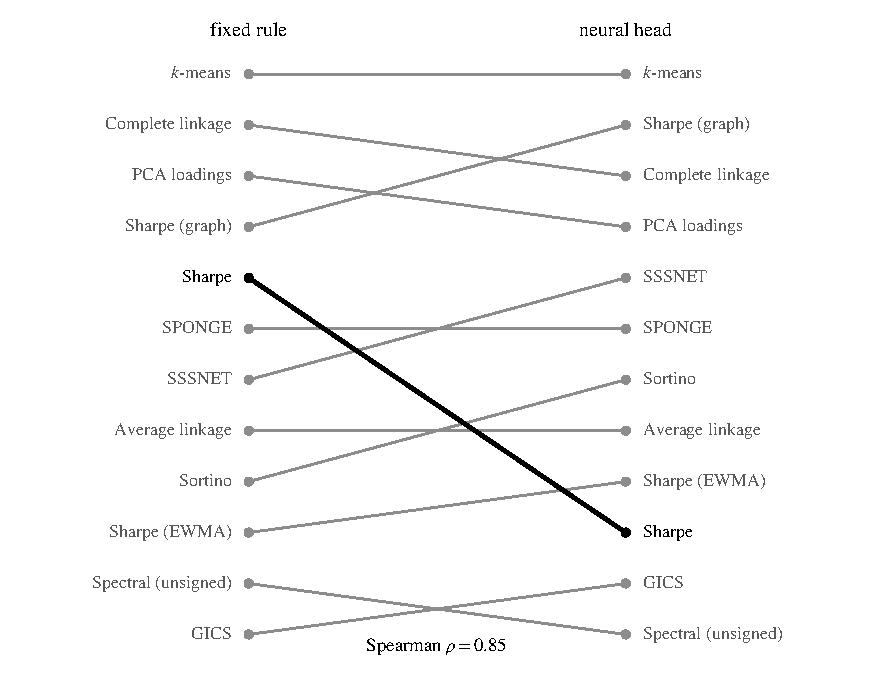
\includegraphics[width=\linewidth]{fig_rank_shift}
\caption{Sharpe-ratio ranks in the rule-based and trained components. This figure plots the 12 clusterizers ranked by Sharpe ratio in each trading component, on the common 60-day estimation window over the $6{,}913$-day sample. The trained column uses the mean per-seed Sharpe ratio over the five head seeds. A clusterizer that changes rank by three places or more is drawn in black. The Spearman rank correlation between the columns is $+0.85$.}
%%  fig_rank_shift regenerated on the v3 matched basis at the 6,913-day
%%  calendar (2026-08-24, Code Branch batch; leader/bottom gate passed).
%%  Caption and figure agree at +0.90.
\label{fig:rank_shift}
\end{figure}

In the trained component, the random control no longer earns a higher Sharpe ratio than the $\K=1$ control. In the rule-based component, where the portfolio is a deterministic function of the partition, the random control earns a higher Sharpe ratio than the $\K=1$ control, $0.89$ against $0.83$. In the trained component, the two controls have the same mean per-seed Sharpe ratio, $1.28$.\footnote{On the seed-averaged payoff, the random control's Sharpe ratio exceeds that of the $\K=1$ control by $0.04$, at $1.50$ against $1.46$.} When we pair the two controls by head seed, the mean difference in Sharpe ratio is $0.00$ ($t = 0.00$). Its standard deviation across the five head-seed runs is $0.08$. The sign of the difference changes from one head-seed run to another, so the two controls are indistinguishable in the trained component. Relative to no partition, a wrong partition therefore does worse in Sharpe ratio in the trained component than in the rule-based component. One explanation, consistent with \secref{sec:hedge}, is that the fixed rule bets small, equal amounts on every stock, so the noise that a random partition adds largely cancels. In this explanation, a trained model fits the structure that the group labels imply, even when that structure is absent or wrong.

%%---------------------------------------------------------------------
%%  §6 DRAFT, 2026-08-16. Yours to edit. All numbers recomputed on the
%%  matched w60 set with the aligned calendar (NEWSTATS_hedge_w60.md,
%%  sections "§6 battery" and "Between-layer rank agreement").
%%
%%  SUPERSEDED, do not restore:
%%    +3.2632 / 21 of 21 / median 1.0439 "leaves the second moment where
%%    it was"  -> old 21-arm mixed set, same-day join. On this paper's
%%    basis the model RAISES vol 15-26%; the licensed mirror claim is
%%    "mostly return, much less risk reduction".
%%    Spearman +0.8390 "the ordering largely survives" -> inflated by
%%    window twins in the 18-arm set. Matched: +0.38, p=0.22. The old
%%    scaffold's ban on "does not survive" is LIFTED for this set; the
%%    drafted wording says "indistinguishable from no agreement".
%%  ⛔ still banned: any individual head-lift point value (bound +0.74
%%    to +1.50, window-mismatched); "the model lifts weak clusterizations and
%%    lowers strong ones" as attribution (window confound, disclosed in
%%    the caveat paragraph instead).
%%  ⚠ 6.3's explanation sentence ("bets small amounts everywhere and the
%%    noise partly cancels") is INTERPRETATION, not measured; soften or
%%    cut if it reads as a claim.
%%---------------------------------------------------------------------
